\documentclass{standalone}
% Load any packages needed for this document
\begin{document}

\section{Chapter 3: Introduction into Computer Graphics}

\subsection{Introduction}

\begin{itemize}
	\item Quick development in computer graphics: from `an expensive toy' to an `attractive research field'
		\begin{itemize}
			\item main reason: human receives most of the information through the \textbf{visual perception channel}
			\end{itemize}
	\item Rapid development concerning hardware, software, and applications
		\begin{itemize}
			\item graphics can be easily accessed and understood by different cultures/people/languages (high synergy among people)
		\end{itemize}
\end{itemize}

\subsection{Why do we need Computer Graphics?}

\begin{itemize}
	\item why graphic $>$ text?
		\begin{itemize}
			\item The representation of texts is also a special form of graphics
			\item Human being seems to have a better access to images and pictures than letters and numbers
				\begin{itemize}
					\item e.g. complex simulation results by visualization or logo of a company
				\end{itemize}
		\end{itemize}
\end{itemize}

\subsubsection{Computer Graphics and Picture Recognition}

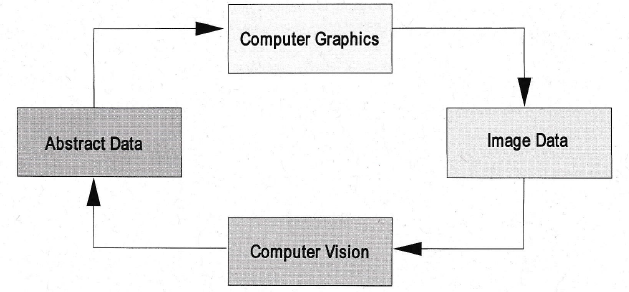
\includegraphics[scale=0.6]{3_1}

\begin{itemize}
	\item When a human perceives the surrounding world, the brain generates an abstract ``data model" $\rightarrow$ same for computers
	\item Computer Vision: extract relevant data out of existing graphics or images
	\item Computer Graphics: display abstracted data as a image
\end{itemize}

\subsection{Applications of Computer Graphics}

\subsubsection{CAD}

\begin{itemize}
	\item one of the most important application 
	\item construction vs design
		\begin{itemize}
			\item Construction (Functional Design)
				\begin{itemize}
					\item the requirements to an assembly part are well defined by function and dimension
					\item all drawings on a CAD system are a \textbf{complex relationship between dimensions, constraints, and material properties}, which describe a part very well
				\end{itemize}
				\item Design (Aesthetic Design)
				\begin{itemize}
					\item \textbf{do not focus on the dimension of a part}, but factors like ergonomics or aesthetics
				\end{itemize}
			\item many suppliers of design software try to combine the relatively free aesthetic design field with the very compulsory functional design, but hasn't been successful due to difficult exchange of data between both worlds
		\end{itemize}
\end{itemize}

\subsubsection{Gaming}
\begin{itemize}
	\item Caused a significance increase of graphic performance in the \textbf{private computer sector}
	\item Cheap components and fast, high-quality software were developed due to the growing demands of players and the competition of the industry
\end{itemize}

\subsubsection{Visualization}

\begin{itemize}
	\item Visualization is the ancestor of 3D computer graphics
	\item \textbf {Definition: Visualization addresses special properties of human perception to visualize and to represent information, which is extracted from large amount of data}
	\item Visualization intends to:
	\begin{itemize}
		\item display structures, models, trends, anomalies, and relationships
		\item give an overview of large amounts of data
		\item give support by means of an easy modification of parameters when searching for interesting regions in a large data field
	\end{itemize}
	These points can be summarized in the mantra of Ben-Shneiderman:
	\begin{center}
	\textbf{overview, zoom-in, filtering, details on request}
	\end{center}
	Thus, a good visualization has the following properties:
	\begin{itemize}
		\item it \textbf{prevents misinterpretation} and ambiguity
		\item it \textbf{optimizes the perception} of subtle properties
		\item it allows displaying \textbf{more data} at a time
	\end{itemize}
	\item Typical data sets which need to be visualized very often:
	\begin{itemize}
		\item MRI: the density can be visualized by different colors and transparencies + cutting plane
		\item CFD: the location and the direction of movement of points with 6 DOF, color and particles, size or shape can display the information
		\item Financial Data: display in a diagram, so that a user can see \textbf{correlations} between variables
		\item CAD (3D data with additional information for edges, corners, surfaces, and surface properties. Complex data structures are used because the data is used not only for visualization but also for other processes. Complexity of the models strongly depends on the display quality)
		\item Statistical data sets (the correlation between different parameters only can be seen through visualization)
	\end{itemize}
	\item Different kinds of visualization in the following table. The different categories do overlap in many cases, "Illustration" has an exceptional position since it can be used everywhere
\end{itemize}

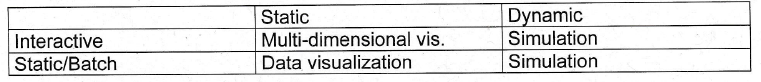
\includegraphics[scale=0.7]{3_8}

\begin{itemize}
	\item Data Visualization
		\begin{itemize}
			\item The most common way would be Excel-like presentation (e.g. pancake diagram, 3D graphs)
		\end{itemize}
	\item Cybernetic Visualization (Simulation)
		\begin{itemize}
			\item The main interest in the visualization of a cybernetic application: speed and possible detection of errors and irregular behavior of the simulated system
			\item The classical way: showing data in a 2D graph as a time-dependent value
		\end{itemize}
	\item Multi-dimensional Visualization
		\begin{itemize}
			\item when much data has to be displayed simultaneously within one image
			\item every point in the space can represent 3 independent values + color, line thickness, transparency, different shapes, etc.
			\item other ways exist but a compromise has to be made concerning the simplicity (e.g. switch between different data visualization planes on any given point of a curve or shape)
		\end{itemize}
	\item Statistics
		\begin{itemize}
			\item typically statistics contain many different values for one single measurement.
			\item the visualization's task is showing possible correlations among the different values
			\item only valid for the given constraints
		\end{itemize}
\end{itemize}

\subsubsection*{Illustration}

\begin{itemize}
	\item Illustrations are 2D add-ons to a 3D object. They contain much additional information about the 3D representation.
	\item GUIs
		\begin{itemize}
			\item the most important means of communication between the user and the computer
			\item the most important input device is the mouse
			\item basic idea of GUI: pointing on an object is one of the easiest gestures of a human being
			\item within the GUI an icon is a small image, which is a representation for a program sequence or for the content of a defined type (they made working with a computer much faster and more comfortable because people can just 'click' on them instead of entering complex instructions)
		\end{itemize}
	\item Fonts
		\begin{itemize}
			\item within the visualization, text is used to assign abstract contents like titles, classifications, or dimensions to a graphical object
			\item Typesets and fonts are the medium of text (based on typography and applications)
		\end{itemize}
	\item Layout
		\begin{itemize}
			\item By placing graphical elements on a surface, the underlying information is structured more clearly and more detailed
			\item typical applications: windows-based desktops such as MacOS, Windows (e.g. word wrap)
			\item Another kind of layout is characterized by the given application (e.g. simulation of operation elements in a car- the ergonomic placement of the elements is essential for the overall handling of the vehicle)
		\end{itemize}
	\item Drawings
		\begin{itemize}
			\item very often used to visualize abstract situations
			\item e.g. organization charts or flowcharts, manuals
		\end{itemize}
	\item Instructions
		\begin{itemize}
			\item instructions consist of a mixture of text, graphical visualization, photos, etc.
			\item very often they visualize products in an abstract and simplified way
			\item e.g. service manuals, assembly manuals
		\end{itemize}
\end{itemize}

\subsection{Definition of 3D Graphics}

\begin{itemize}
	\item Definition of 3D graphics: \textbf{The field 3D graphics deals with the generation of 3D objects and their representation on a two-dimensional surface(e.g. a screen)}
	\item the main focus is on projection and visualization of a 3D space on a 2D surface of any kind
	\item example of 3D graphic devices: video camera, photo camera
	\item main characteristics of 3D graphics:
	\begin{itemize}
		\item data acquisition / data transfer / storage
		\item transformation / processing
		\item data display on 2D
		\item input and output
	\end{itemize}
	\item simple pipeline for data processing: \\
		$\rightarrow$ Definition of geometry as digital data \\
		$\rightarrow$ Processing and transformation of data \\
		$\rightarrow$ Transformation of data to 2D \\
		$\rightarrow$ Display of the results on a screen
\end{itemize}

\subsection{Rendering Pipeline}

\begin{itemize}
	\item The rendering pipeline is the basis for almost every application in computer graphics
	(can be slightly modified for special applications such as augmented reality)
	\item The simplest form of the rendering pipeline: \\
	$\rightarrow$ Processing and transformation of data \\
	$\rightarrow$ Transformation of data to 2D \\
	$\rightarrow$ Display of the results on a screen
	\item transformation / processing: modify the original data in such a way that it can be displayed well on a 2D surface. contains data modified by the user e.g. modified viewing angle onto the geometry
	\item transformation of data to 2D: all modified data has to be transformed onto the 2D surface. e.g. removal of hidden objects or surfaces, transferring a curved surface into triangles, or the integration of illumination models
	\item input/output: reduce the amount of data so that the image can be optimally displayed on the output device (due to limitation in resolution)
\end{itemize}

\subsection{Definition of Geometry in the Computer}

\begin{itemize}
	\item Algorithms for a geometric representation of curves and bodies were developed in order to model hulls, car bodies, and fuselages
	\item B\'ezier developed a CAD-system (further developed into the 'UNISURF' system later on), close approximation to geometry
	\item In order to define geometry, the information should be sufficient but not redundant
	\item It can be distinguished between volumetric and surface models
\end{itemize}

\subsubsection*{Discrete Definition of Surfaces}
\begin{itemize}
	\item Cloud of Points:
	\begin{itemize}
		\item the simplest model, every point of the cloud is defined by its coordinates
		\item The point cannot be rendered(no information on color or texture) and there is no connectivity among the points(separate parts cannot be selected in the model)
		\item 3D-scanner typically provides a cloud of points
		\item difficult to create a good surface out of the clouds of points because the acquired data is noisy and erroneous
	\end{itemize}
	\item Polygons, Tessellation:
	\begin{itemize}
		\item Tessellation is a method for defining or generating a mesh of geometric basic elements(polygons), which approximate a complex surface
		\item Polygon, especially triangle, is one of the most important basic elements of computer graphics
		\item "triangulation": the process in which a free-form surface is transformed into triangles (The mesh approximates the surface by triangles and reduces the complexity)
		\item additional data has to be considered when rendering (e.g. perpendicular of a surface)
	\end{itemize}
	\item Polystrips
	\begin{itemize}
		\item when a point is added to a triangle, a second triangle will be generated
		\item advantage: a large amount of surfaces can be generated by a very low amount of data
		\item stored in two tables: the point(vertex) table with all coordinates of the triangle's corners and the strip table with all coherent triangles
		\item details could be lost since any curve is approximated by straight lines of different lengths
		\item many times the triangulation is done at a very late stage in rendering because often working with mathematically exact representations of the geometry is required
	\end{itemize}
\end{itemize}

\subsubsection*{Mathematical Description of Geometries}

\begin{itemize}
	\item Typically, the surfaces of objects are represented by approximating functions
	\item A parametric representation is used for the approximation or interpolation of these surfaces (e.g. parametric polynomials - B\'ezier, B-Spline)
	\item Surface models are mainly used- drawback: there are no relationships among the individual parts of the surface (The individual surfaces are not correlated with an object and thus the shape of an object is a question of interpretation)
	\item possibilities for the mathematical description of curves and surfaces: explicit, implicit, parametric
	\begin{itemize}
		\item explicit: $y = f(x)$
		\begin{itemize}
		  	\item only one value for y is associated with the variable x
		  	\item thus problems arise for closed curves or objects
		  	\item it is not invariant to rotations
		  	\item only a few geometries can be described by such an explicit notation, rarely used
		\end{itemize}
		\item implicit: $f(x, y) = 0$
		\begin{itemize} 
			\item typically implicit equations have more solutions than required and thus additional constraints have to be considered 
			\item also rarely used in virtual reality
		\end{itemize}
		\item parametric: $Q(t) = (x(t), y(t)$
		\begin{itemize}
			\item the most common descriptive form
			\item no equivocations could occur, the definition is invariant to rotations
			\item infinite slopes can be described by tangential vectors which are finite
			\item typically consist of rational polynomials of the nth degree, most frequently cubic polynomials are used
			\item any point of the geometry can be exactly determined by mathematical functions (particular interest for CAD)
		\end{itemize}
	\end{itemize}
	\item B\'ezier splines:
	\begin{itemize}
		\item first used in shipyards
		\item goal: interconnect given points by a smooth line
		\item points that approximate the curve are called ``control points"
		\item mathematical function that delivers the result is named "base function", guarantees that the requirement for continuity in the control points is kept by interpolation or approximation
	\end{itemize}
	\item approximation: a curve approximates given control points / interpolation: the calculated curve has to meet the control points exactly; important in both cases that continuity is fulfilled
	\item ``parametric continuity":
	\begin{itemize}
		\item represented by the letter C and its exponent i which defines the degree of the i\textsuperscript{th} derivation \\
		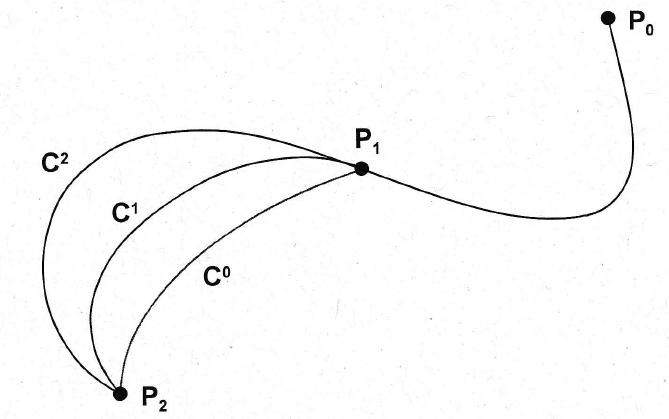
\includegraphics[scale=0.5]{3_24}
		\item C\textsuperscript{0} continuity: guarantees that the curve is not interrupted, but it could happen that a curve is not smooth in the point P1 but has an edge instead
		\item C\textsuperscript{1} continuity: the first derivation is continuous, all tangent vectors in the point P1 have the same slope, the curve is smooth at the point P1 (continuity of tangents)
		\item C\textsuperscript{2} continuity: the second derivation is continuous, the curve looks even smoother, also named as continuity of curvature
	\end{itemize}
\end{itemize}

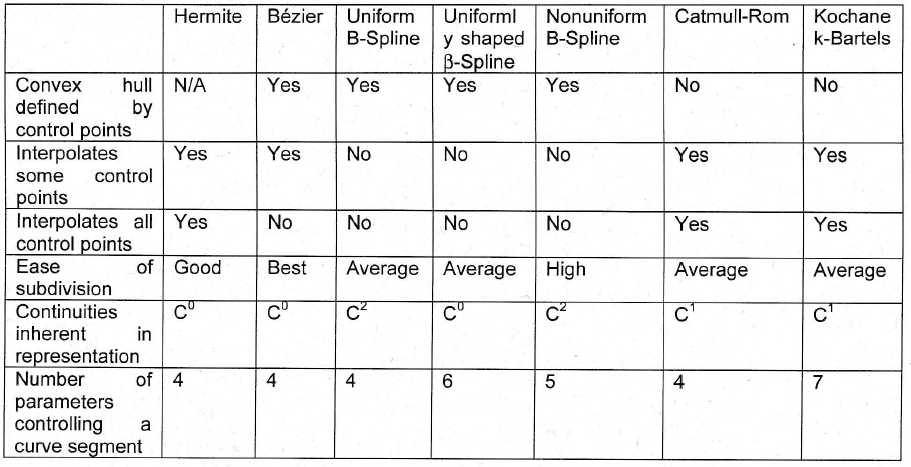
\includegraphics[scale=0.6]{3_25}

\subsubsection*{Approximating Splines}

\begin{itemize}
	\item If an approximating curve is described by control points, there is an additional requirement that the resulting curve has to be within the polygon shaped by the control points
	\item The shape is a complex polygon that encloses all control points like a rubber band
	\item If the control points are extreme points, they are part of the polygon; otherwise, they are inside of the polygon
	\item The complex shape allows a good control of the curve (guarantees the curve is always within the visible area)\\
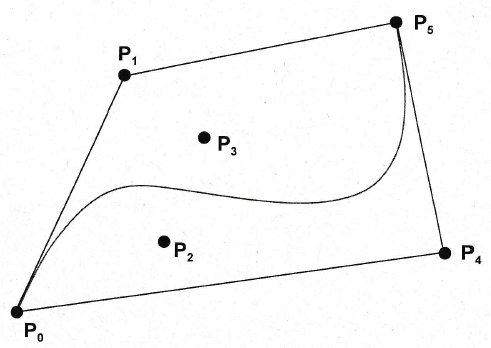
\includegraphics[scale=0.5]{3_26}
	\item B\'ezier Curve
	\begin{itemize}
		\item the base function is defined in a parametric form Q(t), t is a variable within [0, 1)
		\item the base function depends on the amount of control points; the whole curve is changed by just changing one point
		\item in addition to B\'ezier curve, also the first and last control point belong to the curve Q(t)
		\item always inside a complex polygon, because at least three control points are extreme points
		\item The Algorithm of de Casteljau (iterative):
			\begin{itemize}
				\item The base function of a B\'ezier curve can be calculated by the algorithm of de Casteljau
				\item idea: choose t and subdivide the first line b\textsubscript{0}b\textsubscript{1} at the distance t

				\begin{equation}
					b\textsubscript{0}\textsuperscript{1}(t) = (1-t)b\textsubscript{0}+t b\textsubscript{1}
				\end{equation}
				\item This process is repeated for the lines b\textsubscript{1}b\textsubscript{2} and b\textsubscript{2}b\textsubscript{3}, until in total three new points b\textsubscript{0}\textsuperscript{1}, b\textsubscript{1}\textsuperscript{1}, b\textsubscript{2}\textsuperscript{1} will result 
				\item the calculation is repeated with the three new points and so on 
				\item In general:

				\begin{align}
					b\textsubscript{i}\textsuperscript{r}(t) &= (1-t)b\textsubscript{i}\textsuperscript{r-1}+t b\textsubscript{i+1}\textsuperscript{r-1}
					b\textsubscript{i}\textsuperscript{r}(t) &= b\textsubscript{i}
				\end{align}

				where $i =$ number of control points; $i=0,\dots,(n-r)$, $r =$ number of lines; $r=1,\dots,n$
			\end{itemize}
			
			\begin{figure}[H]
				\begin{subfigure}[b]{0.3\textwidth}
					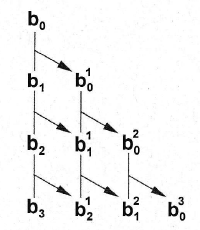
\includegraphics[width=\linewidth]{3_29} 
				\end{subfigure}
				\begin{subfigure}[b]{0.65\textwidth}
					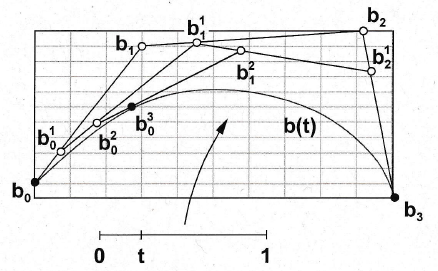
\includegraphics[width=\linewidth]{3_30}		
				\end{subfigure}
			\end{figure}
	\end{itemize}
	
	\begin{itemize}
		\item For a better approximation of the curve, more control points have to be used which will increase the computing time
		\item The algorithm of de Castelijau can also be used, if more than four control points exist
		\item The number of control points(L+1) defines the kind of curve
		\item For L=3 (cubic B\'ezier curve), it is further elaborated and simplified as:
		\begin{equation}
			Q(t) = b\textsubscript{0}(1-t)\textsuperscript{3}+b\textsubscript{1}3t(1-t)\textsuperscript{2}+b\textsubscript{2}3t\textsuperscript{2}(1-t)+b\textsubscript{3}t\textsuperscript{3}
		\end{equation}
		\item Bernstein Polynomials: \\
		B\'ezier curves can be more easily calculated by using it; do not work recursively but directly deliver the result at the position t by using polynomial coefficients \\
		When (L+1) control points are given, the function is defined by:
		\begin{equation}
			Q(t) = \sum_{i=0}^Lb\textsubscript{i} B\textsubscript{i}\textsuperscript{L}(t)
		\end{equation}
		$$ B\textsubscript{i}\textsuperscript{L}(t) $$ is the Bernstein polynomial, which is defined as:
		\begin{equation}
			B\textsubscript{i}\textsuperscript{L}(t)= \textsubscript{L}C\textsubscript{i} (1-t)\textsuperscript{L-i}t\textsuperscript{i}, \quad L >=i
		\end{equation}
	\end{itemize}
	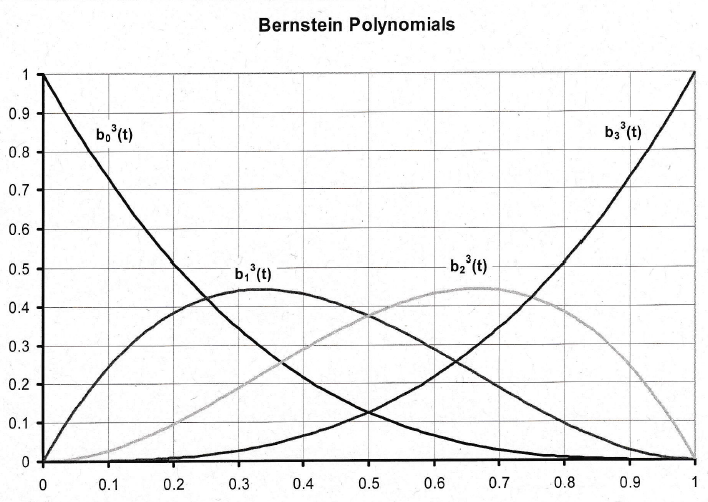
\includegraphics[scale=0.65]{3_31}
	\begin{itemize}
		\item If B\'ezier curves of a high degree are employed, it is difficult to keep the curve smooth
		\item Bernstein polynomials can also be calculated by a successive superposition of linear B\'ezier splines
	\end{itemize}
	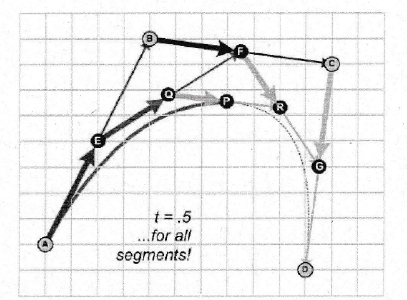
\includegraphics[scale=0.8]{3_32}
\end{itemize}

\subsubsection*{Interpolating Splines}

\begin{itemize}
	\item Boundary Representation - B-Rep
	\begin{itemize}
		\item Edge representations(or surface models or boundary representation) use 3D polygons to define the limiting surfaces of an object \\
		The limiting surfaces can be plain surfaces, but also surfaces of higher order \\
		It allows an exact mathematical description for many geometries, good approximation for the others
		\item B-Rep models consist of three object types: surfaces, edges, and corners
		\item To create on object out of the individual surfaces, the data structure must also contain a topological part(which defines the neighborhood of the surfaces) beside the normal geometric definition \\
		very common topological list contains 4 parts: a list of points/edges/surfaces/volumetric objects \\
		This list corresponds to a point-edge-surface model \\
		advantage: compact storage of all defining elements, since every point has to be stored only once
		\item The advantage of surface models consists in the complete availability of all topological information \\
		Surfaces, edges, and points can be stored as individual objects, which significantly increases the flexibility of the object \\
		one drawback: high calculation effort and complex network structure
	\end{itemize}
\end{itemize}

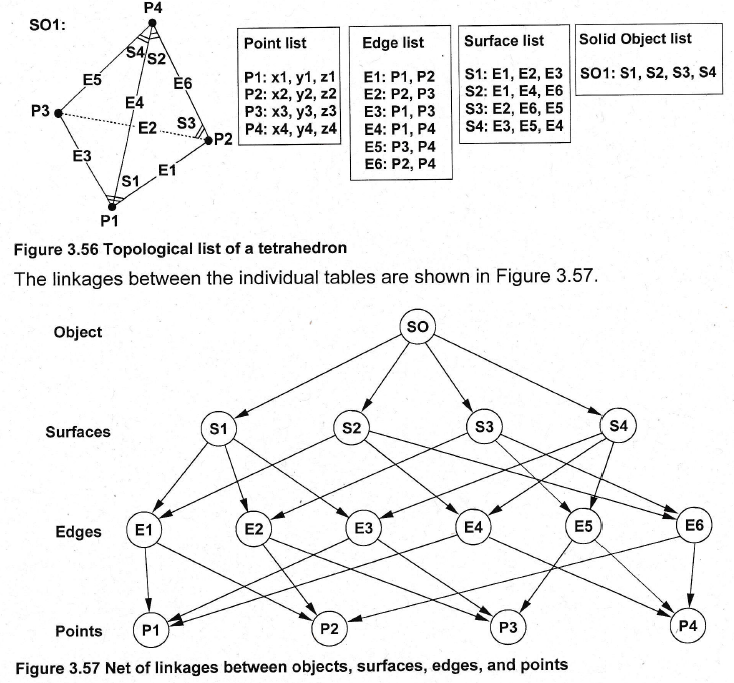
\includegraphics[scale=0.7]{3_56}

\subsubsection*{Volumetric Models}

\begin{itemize}
	\item The goal is to create objects that can be generally used 
	\item Only complete representations of physical objects are accepted
	\item Volumetric models can be distinguished into: 
		\begin{itemize}
			\item cell models: discretize the required space of the object 
			\item accumulative models: the object consists of a sum of basic elements 
			\item generative objects: predefined volumetric elements (primitives) and Boolean operations on the elements 
			\item other models: parametric models(e.g. CAD), sweep models, breakdown into elements(FEM)
		\end{itemize}
	\item CSG(Constructive/Computational Solid Geometry)
	\begin{itemize}
		\item 3 primitive methods to shape geometry out of simple objects: merging parts(set union), cutting parts out(difference), calculate common parts of objects(intersection) $\rightarrow$ this approach is used by CSG
		\item CSG uses simple basic geometries like cones, spheres, cubes which are completely described by mathematical functions
		\item Complex objects can be described by a tree of Boolean operations		
	\end{itemize}
	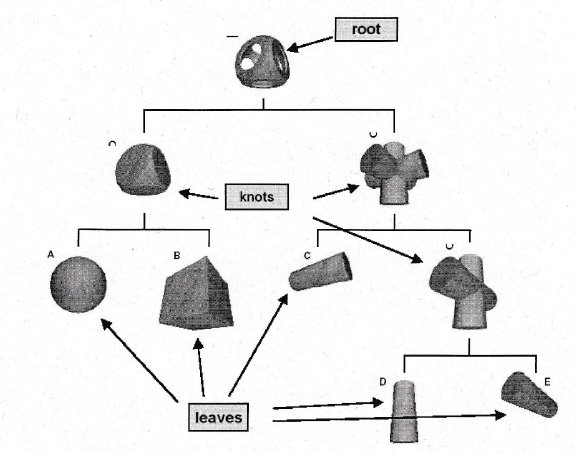
\includegraphics[scale=0.8]{3_62}
	\item Cell Models
	\begin{itemize}
		\item In analogy to pixel models, cell models use \textbf{voxels(volume elements)} of uniform size to represent volumetric models
		\item the voxels are arranged in a regular 3D grid and are represented by the coordinates of the cell's center
		\item the maximum resolution is defined by the cell size
		\item the representation of 3D objects using cell models is suitable for the computation of volumes and other Boolean operations; however the geometrical elements(corner, edge, surface) can only be represented imprecisely or with a large effort
	\end{itemize}
\end{itemize}

\subsection{Color Definitions in the Computer}

\subsubsection*{Color Depth and Color Palettes}

\begin{itemize}
	\item The maximum number of colors to be used by the computer is defined by the color depth, i.e. the amount of bits that describe a color
	\item (number of colors) = $2^{color depth}$ (e.g. color depth 1 means 2 colors can be used)
	\item If the color depth is smaller than 8 bits, color palettes(color look-up tables, LUT) are used
	\begin{itemize}
		\item color palettes: an array in which each entry defines exactly one color
		\item thus, this array contains color information for each pixel
	\end{itemize}
	\item In the picture memory, references to the LUT exist
	\begin{itemize}
		\item if colors change, the entry in the LUT is modified while the picture memory stays unchanged
	\end{itemize}
	\item Each entry in the look-up table consists of a tuple of numbers for the colors RGB
	\item If the color depth is larger then 8 bits, the color look-up table would become too large and thus color information is directly stored in the picture memory
\end{itemize}

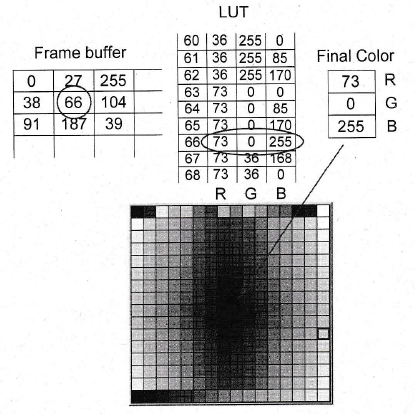
\includegraphics[scale=0.7]{3_64}

\subsubsection*{Color Quantization}

\begin{itemize}
	\item Color Quantization: to reduce the required memory for displaying images
	\begin{itemize}
		\item Due to the immense costs of memory chips, the available graphic memory was restricted for a long time
		\item Thus, old graphic cards could only display images with a color depth of 8 Bit with a poor resolution
		\item Images with a higher color depth had to be reduced to 8 Bit color depth
		\item Even today it is used e.g. graphics which are transferred over the Internet, are compressed in color to diminish the time for transmission
		\item Furthermore, human's eye can resolve a limited amount of different colors(color resolution from 5-8 Bits per color) so images can be reduced in color depth without being noticed by the user
	\end{itemize}
	\item Need for high color depth: typical images with a color gradient or antialiasing are only possible with a higher color depth
	\item The colors in the original image, which will be assigned to be the same color in the color palette, form a cluster(= color domain) \\
	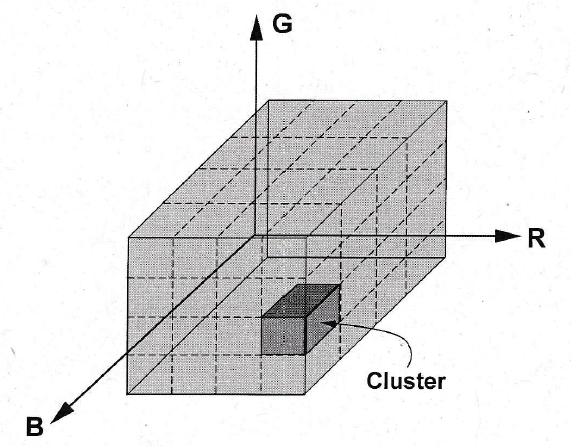
\includegraphics[scale=0.4]{3_66}
	\item Pre-clustering procedure:
	\begin{itemize}
		\item divides the color space into a certain amount of clusters
		\item the color of a cluster is one color of the color palette
		\item RGB color space is uniformly divided into 256 colors without considering whether the colors exist in the real image or not
		\item this method delivers unsatisfying outcomes
	\end{itemize}
	\item Popularity algorithm:
	\begin{itemize}
		\item one of the algorithms to create an adapted color palette
		\item a histogram of colors is created: it is examined how often every color exists in the original image \\
		$\rightarrow$ A new color palette is generated out of m(=number of the desired color depth, e.g. 256) mostly used colors \\
		$\rightarrow$ the colors of the new palette are associated with the original colors of the image i.e. the colors of the palette which fit best the original color \\
		$\rightarrow$ the rest of the image colors is replaced by the one from the palette, which is very close to it (to determine the most similar color, the Euclidian distance is calculated)
		\item drawback:\\
		very time consuming; no structure is created so the complete color palette has to be searched for every color assignment \\
		any color details in small segments of the image could be completely wrong
	\end{itemize}
	\item Median-cut algorithm:
	\begin{itemize}
		\item In order to find the colors for the adapted color palette, the best approximation of the available colors is created instead of choosing colors from the original image
		\item all colors from the original image are marked in the RGB color cube \\
		$\rightarrow$ the cube is reduced in size until the cloud of marked colors fits the cube best \\
		$\rightarrow$ the cube is cut parallel to its longest edge(median-cut) in such a way that every sub-cube contains the same number of pixels \\
		$\rightarrow$  both sub-cubes are contracted until they fit exactly the number of pixels \\
		$\rightarrow$ again, the sub-cubes are cut along the median line and procedure recurs \\
		The procedure stops when a previously defined number of cub-cubes is reached
		\item in the best case, the resulting segments of the RGB color cube contain only one color that can be assigned to the pixels
		\item if more than one color is in the final cube, a mean value is calculated
	\end{itemize}
\end{itemize}

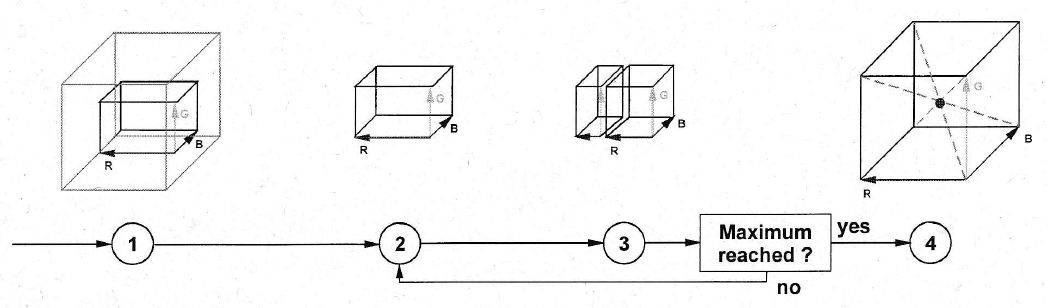
\includegraphics[scale=0.5]{3_69}

\begin{itemize}
	\item after the determination of the color palette, the difference(failure) between the needed(real) color and the associated color of the palette is not taken into account
	\item Floyd-Steinberg algorithm:
	\begin{itemize}
		\item in order to remove the remaining color steps, smoothens the color transitions
		\item the algorithm spreads this failure to the point of the neighborhood with the following weight: \\
		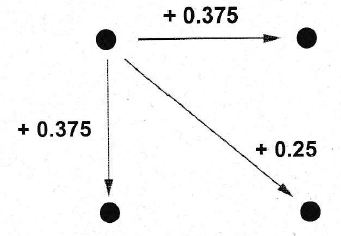
\includegraphics[scale=0.5]{3_71}
		\item the failures are gradually spread over the complete image without increasing the possible amount of palette colors
	\end{itemize}
\end{itemize}


\setcounter{subsection}{9}
\subsection{Calculation of Object's Visibility}

\begin{itemize}
	\item \textbf{visibility problem}: correct selection of polygons for a 3D scene, which are visible from a given view point
		\begin{itemize}
			\item only a small amount of polygons are visible.
			\item but viewpoint change rapidly $\rightarrow$ \textbf{real-time selection} is crucial
			\item algorithms for the object space vs. algorithms for the image space
				\begin{itemize}
					\item object space: work on the level of the objects with the same accuracy the objects have.
					\item image space: work on the level of the rasterized image with a resolution of one pixel
				\end{itemize}
		\end{itemize}
	\item \textbf{Culling procedure}: calculate the invisible lines and surfaces of the objects in a scene.
		\begin{itemize}
			\item view frustrum culling: all objects outside the viewing cone will be removed
			\item back face culling: the back faces of an object are removed
			\item occlusion culling: all objects that are hidden by an other one, are removed
		\end{itemize}
\end{itemize}

\subsubsection{View Frustrum Culling}

\begin{itemize}
	\item using a view cone: all objects inside frustrum have to be calculated. objects are on the border of the frustrum will only be partly calculated
\end{itemize}

\begin{figure}[H]
	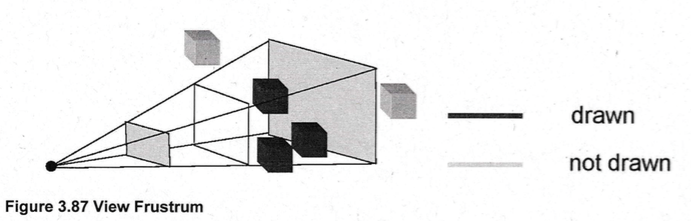
\includegraphics[width=\linewidth]{3_87}
\end{figure}


\subsubsection{Back Face Culling}

\begin{itemize}
	\item surfaces of an object facing away from the user will be removed
	\item z-component of the polygon's perpendicular has to be checked. (positive: faces away from the user - invisible)
\end{itemize}

\begin{figure}[H]
	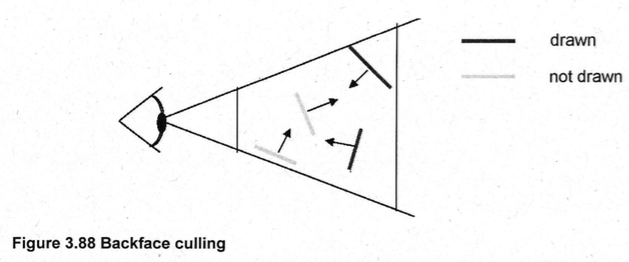
\includegraphics[width=\linewidth]{3_88}
\end{figure}


\subsubsection{Occlusion Culling}

\begin{itemize}
	\item all objects which are completely hidden by other objects from a given viewpoints are removed
	\item in principle, depth information is used for occlusion culling.
\end{itemize}

\subsubsection*{Priority Algorithms (painter algorithm)}

\begin{itemize}
	\item surfaces of an object are sorted concerning their depths, and displayed from the back to the front. (only elements on the top are visible)
	\item every surface has to be checked. 
\end{itemize}

\subsubsection*{Ray Tracing Algorithms (Ray Casting)}

\begin{itemize}
	\item rays from the center of projection into the scene are traced. (for every pixel in the image plane)
	\item intersection points of a ray with an object are calculated:
		\begin{itemize}
			\item tracing a ``light ray" in the backward direction from the center of projection to a pixel in the scene.
			\item determining the pixel's color by looking up the color of the hidden object in the scene.
			\item if a pixel does not have any intersection point, it will have the same color as the background.
			\item in all other cases, the intersection point is calculated, which is closest to the image plane.
		\end{itemize}
	\item +) for properties such as transparency and reflection, the color value of a pixel could be calculated. (raytracers)
\end{itemize}


\subsubsection*{z-Buffer Algorithm}

\begin{itemize}
	\item z-value (depth) of the displayed point is also stored:
		\begin{enumerate}
			\item all value of the depth buffer is set to $(-) \infty$
			\item for each surface of a polygon, depth info. of every point in the plane is calculated. At first, calculate for the corner points then arbitrary point in the middle of a polygon defined as follows:
			
			\begin{equation}
				z = \frac{-D - Ax - By}{C}
			\end{equation}
			
			\item if the depth of a calculated pixel is smaller than the value that is already stored, update to the newly calculated value.
			\item iterate 2, 3 for every polygons
		\end{enumerate}
	\item benefits:
		\begin{itemize}
			\item the order of the sampled polygons is arbitrary.
			\item the algorithm is independent of the complexity of the individual objects. 
			\item it is possible to add objects into scenes that are already rendered.
			\item the slow algorithm can be accelerated by implementing it into hardware
		\end{itemize}
	\item drawbacks:
		\begin{itemize}
			\item a large amount of memory is needed $\rightarrow$ solution: can be reduced by dividing the image into multiple rectangles and separately calculating. (parallel)
			\item exact smoothing, reflection and transparency are not possible. (object per pixel can be stored) $\rightarrow$ solution: every pixel is divided into n x n sub-pixels and edge is calculated on the level of the sub-pixels. An average color is calculated from the sub-pixels. 
			\item limited resolution. Object with a large extension in depth, sometimes the same value of z appears.
		\end{itemize}
\end{itemize}

\begin{figure}[h]
	\centering
	\begin{subfigure}[b]{0.45\textwidth}
		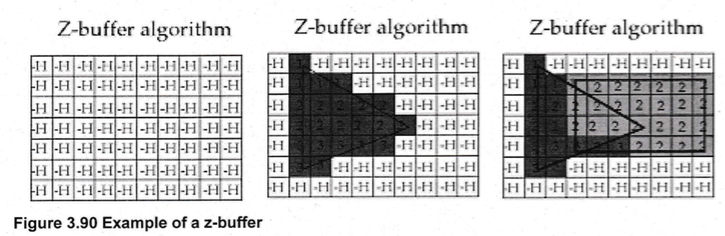
\includegraphics[width=\linewidth]{3_90}
	\end{subfigure}
	\begin{subfigure}[b]{0.45\textwidth}
		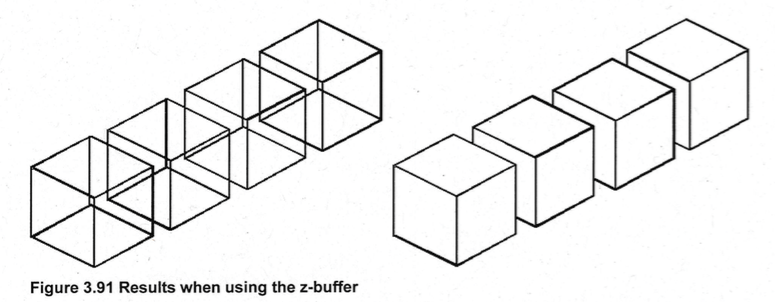
\includegraphics[width=\linewidth]{3_91}
	\end{subfigure}
\end{figure}

\subsection{The Distance Dependent Resolution (Level of Detail)}

\begin{itemize}
	\item the object far from the user $\rightarrow$ no need to simulate details
	\item the object covering the complete field of view $\rightarrow$ has to be displayed with more details
\end{itemize}

\begin{figure}[H]
	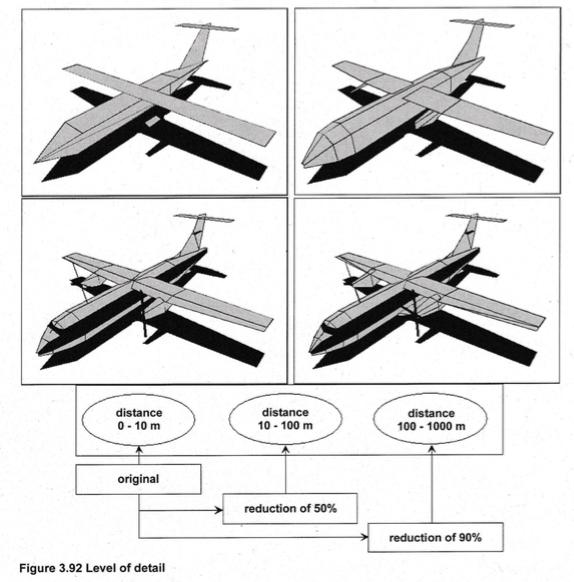
\includegraphics[width=\linewidth]{3_92}
\end{figure}


\subsection{Illumination Models}

\begin{itemize}
	\item photo-realistic quality $\rightarrow$ illumination model
	\item physical properties of light (Figure 3.93)
		\begin{itemize}
			\item diffuse reflection: uniformly scattered into all directions. The intensity depends on the perpendicular of the surface and on the direction of the incoming light.
			\item complete reflection: angle of incoming light = angle of reflected light. (color and the size of the reflection spot depends on the material)
			\item transmission: coupled with refraction. Global illumination models capture transmission.
		\end{itemize}
	\item rendering of light and shadow is affects by			
		\begin{itemize}
			\item light source type
			\item geometry, position of light source and camera
			\item geometry of the light, curvature of the geometry
			\item surface properties of the illuminated scenery (e.g. transparency, color, reflections)
			\item medium that transports the light (e.g. air, fog)
		\end{itemize}
\end{itemize}

\begin{figure}[H]
	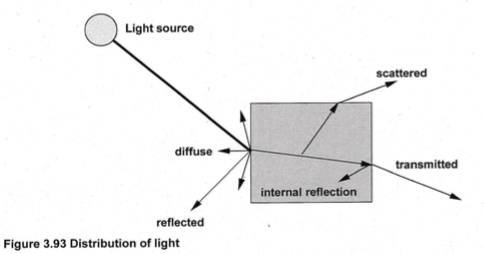
\includegraphics[width=\linewidth]{3_93}
\end{figure}

\subsubsection*{Light sources}

Figure 3.95

\begin{itemize}
	\item ambient light: background illumination. No defined light source and has no direction
	\item distant light: parallel light into one direction. The intensity of the light does not decrease with the distance from the light source
	\item spatial light: parallel light but decreases with the distance. (make smooth shadows)
	\item point light: light into every direction. The intensity decreases with the distance from the light source. (e.g. a simple bulbs)
	\item spotlight: cone-shaped light. The direction, position and dimension of the cone have to be defined.
\end{itemize}

\subsubsection*{Local vs. Global}

\begin{itemize}
	\item two different approaches for calculating the lighting of a scenary. 
	\item local: behavior of one point of the surface depending on the incoming light
	\item global: whole scenery together with the distribution of light
\end{itemize}

\subsubsection{Local Illumination Models}

\begin{itemize}
	\item calculates light intensity of a point on the surface of an object independently. 
	\item fast but many compromises
	\item can be implemented by hardware
	\item light transport:
		\begin{itemize}
			\item ambient light. no direction, uniformly distributed. 
			\item light which reaches the surface of an object and uniformly reflected (in all directions)
			\item light with a defined direction. 
		\end{itemize}
	\item Note: See the figures in the lecture note.
\end{itemize}

\subsubsection*{Reflection with Ambient Light}

\begin{itemize}
	\item light doesn't have orientation and reflected uniformly from every surface
	\item not sufficient for the visualization of object.
	\item intensity:
		\begin{equation}
			I = I_a \cdot k_a
		\end{equation}
		
		where $I_a$ is the intensity of the ambient light and $k_a$ is the ambient reflection factor ($0 < k_a < 1$)
\end{itemize}

\subsubsection*{Diffuse Surfaces}

\begin{itemize}
	\item by point light which emits light into all directions
	\item reflection is regardless of the viewer's position
	\item Lambert's reflection law:
		
		\begin{align}
			I &= I_p \cdot k_d \cos{\theta} \\
			&= 	I_p \cdot k_d (\vec{N} \bold{\cdot} \vec{L})
		\end{align}
		
		where $\vec{N}$ is the normal vector of surface, the $\vec{L}$ points into the direction of the light source, $I_p$ is the intensity of the incoming light and $k_d$ is the diffuse reflection coefficient. ($0 < k_d < 1$)
	\item pale surfaces can be visualized very realistically. However the surface properties of many objects are not suitable.
\end{itemize}

\subsubsection*{Specular Surfaces}

\begin{itemize}
	\item varnished or polished surfaces. (light center reflection - highlights)
	\item depends on the geometry and the viewpoint of the user. (position of the user is important!)
	
	\begin{equation}
		I = I_p \cdot k_s \cos^n{\alpha}
	\end{equation}
\end{itemize}

\subsubsection*{Ambient + Diffuse + Specular}

\begin{itemize}
	\item sum all terms..
	\begin{align}
		I &= \text{ambient} + \text{diffuse} + \text{specular} \\ 
		&= I_a \cdot k_a + I_p \cdot k_d \cos{\theta} + I_p \cdot k_s \cos^n \alpha \\
		&= I_a \cdot k_a + f_{att} \cdot I_p \big(k_d \cdot \cos \theta + k_s \cdot \cos^n \alpha \big) \\
		&= I_a \cdot k_a + f_{att} \cdot I_p \big(k_d \cdot (\vec{N} \bold{\cdot} \vec{L}) + k_s \cdot (\vec{R} \cdot \vec{V})^n \big)
	\end{align}
	
	where the factor $k$ and the exponent $n$ (shininess) depend on the kind of surface and influence the shape of the highlight.
	\item $\cos ^n \alpha$ heuristically approaches the scattering of the reflected light.
	\item attenuation element $f_{att}$: represents the decrease of the light intensity with an increasing distance to the light source ($d_L$): 
	
	\begin{equation}
		f_{att} = \frac{1}{d_L^2}
	\end{equation}
	
	\item refer to Figure 3.101
	\item note that the model is based on simplified assumptions for the physical properties of the surface. (other factors: microstructure of the surface, transparency of the material, wavelength of light...)
\end{itemize}

\begin{figure}[H]
	\centering
	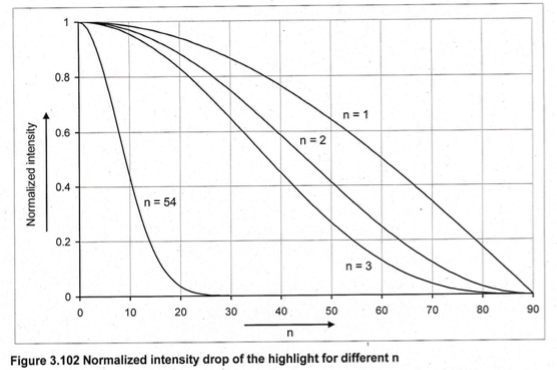
\includegraphics[width=0.7\linewidth]{3_102}
\end{figure}


\subsubsection*{Approximation and Shading methods}

\begin{itemize}
	\item calculating illumination model only for the edges of the triangle, and all points in between are only interpolated. $\rightarrow$ saving time, good approximation to the local illumination model.
	\item flat shading (constant shading): if no apprx. is made between the corners of the triangle.
	\item alternatives: two methods for interpolation - Gouraud and the Phong interpolation 
\end{itemize}

\subsubsection*{Flat Shading}

\begin{itemize}
	\item Figure 3.106
	\item no apprx.
	\item illumination model used for one point of the polygon and all points of the polygon are assigned to the calculated color. 
	\item works well when...
		\begin{itemize}
			\item the light source is infinitely far away ($\theta = \text{const.}$)
			\item the viewer is infinitely far away ($\alpha = \text{const.}$)
			\item polygon represents the true surface of the object and not an approximation of a curved surface (no curved surface)
		\end{itemize}
	\item very fast but not realistic especially for ball.
	\item Mach-effect: two neighboring polygons with different shadings also have different intensities along their common edges. (problem!)
		\begin{itemize}
			\item Figure 3.107
			\item reason why the curved surfaces are not realistic in flat shading
		\end{itemize}
\end{itemize}


\subsubsection*{Gouraud shading}

\begin{itemize}
	\item color and intensity interpolation (apprx.)
	\item does not shade every polygon but treats it as part of a larger surface. (vertices)
	\begin{enumerate}
		\item vertex perpendicular is calculated for every vertex of the polygon grid.
			\begin{equation}
				N_V = \frac{\sum_{i=1}^n N_i}{\abs{n \sum_{i=1} N_i}}
			\end{equation}
		\item illumination model is applied to the vertices 
		\item intensity for the other points of the surface to be shaded by an interpolation of the other vertices.
			\begin{itemize}
				\item intensity for the points on the edges is calculated first by interpolating between the vertices. 
				\item inner area of the polygon can be shaded by interpolating between the intensities of the edges. (scan-line procedure: Figure 3.109)
				
				\begin{align}
					I_a &= I_1 - (I_1 - I_2) \frac{y_1 - y_s}{y_1 - y_2} \\
					I_b &= I_1 - (I_1 - I_3) \frac{y_1 - y_s}{y_1 - y_3} \\
					I_p &= I_b - (I_b - I_a) \frac{x_b - x_p}{x_b - x_a}
				\end{align}
				
			\end{itemize}
	\end{enumerate}
	\item drawbacks: shiny reflections could get lost due to the interpolation $\rightarrow$ Phong shading
\end{itemize}

\begin{figure}[H]
	\begin{subfigure}[b]{0.45\textwidth}
		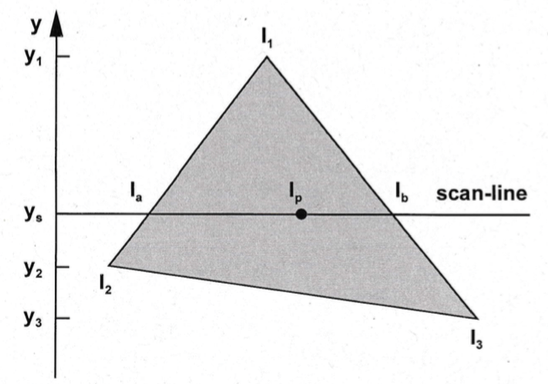
\includegraphics[width=\linewidth]{3_109}
	\end{subfigure}
	\begin{subfigure}[b]{0.45\textwidth}
		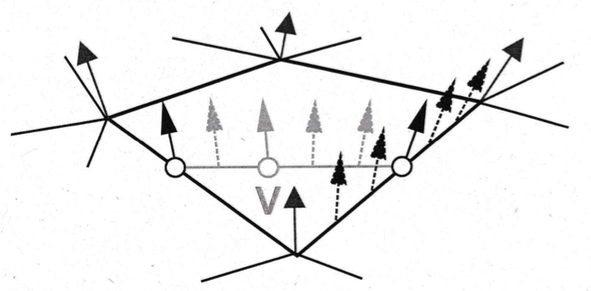
\includegraphics[width=\linewidth]{3_112}
	\end{subfigure}
\end{figure}

\subsubsection*{Phong shading}

\begin{itemize}
	\item interpolation, but perpendiculars of the surfaces are interpolated instead of the intensities.
	\item very realistic but computationally expensive.
		\begin{enumerate}
			\item vertex perpendiculars of the polygon grid are calculated by using the mean value of the perpendiculars of the neighboring surfaces. 
			\item the perpendiculars is calculated by interpolation for every pixel of the surface to be shaded. (sperpendiculars of the pixels on the edges are interpolated from the vertex perpendiculars)
			\item perpendiculars of the inner polygon pixels are calcualted by a scan-line procedure.
			\item normalize and local illumination procedure is applied for every perpendicular. 
		\end{enumerate}
\end{itemize}

\subsubsection*{Interpolation methods}

\begin{itemize}
	\item Phong is time-consuming (more calculation)
	\item Phong is more realistic (more precise illumination)
	\item if the light hits the inner area without illuminating the corner, Gouraud does not work properly (all dark polygon)
	\item For both methods, the silhouette of the polygon is not very smooth. $\rightarrow$ subdividing the polygon into much smaller polygons. (but computation $\uparrow$)
	\item result of shading algorithms with interpolation depend on the orientation of the polygon. (Figure 3.114)
	\item if two neighboring polygons do not have any vertex on a common edge then it's problematic. (Figure 3.115)
	\item the geometry of the surfaces sometimes, is not represented very well by the vertex perpendiculars. In this case, light from very far distance will cause no change in shading. (Figure 3.116)
\end{itemize}


\subsubsection{Global Illumination Models}

\begin{itemize}
	\item consider the complete scenery: the relationship among objects is considered.
	\item very realistic(advantage) but dramatically higher computation time(drawback)
	\item transmission (incl. diffraction) and the exact distribution of diffuse light are global model
	\item cannot implemented in hardware (so many factors e.g. amount of light source, geometry complexity, medium...)
	\item two solution:
		\begin{itemize}
			\item Raytracing: calculate reflection, transparencies, refraction (w/o scattering) and shadows. Diffuse reflection is not supported well.
			\item Radiosity: only for diffuse reflection. (opague or diffuse radiator assumption)
		\end{itemize}
\end{itemize}

\subsubsection{Raytracing}

\begin{itemize}
	\item trace a light beam on its way from the source to the eye. (when calculating, eye to source since only a few light reach the eye)
	\item eye emits rays $\rightarrow$ if the ray strikes a surface it's reflected, changed in color, and partially absorbed. 
	\item uses optical laws for ideal reflection and refraction. 
	\item process stops under the conditions of:
		\begin{itemize}
			\item the ray strikes a light source
			\item the transported energy of the light ray is too low
			\item the ray leaves the scenery
		\end{itemize}
	\item shadow rays: towards the light source are calculated for the place, at which the initial ray hits upon the object. only if no solid object is between, the source illuminates the object directly.
	\item ray is emitted for every pixel until it strikes an object. $\rightarrow$ ray hits upon an object, the local illumination model is applied $\rightarrow$ two new rays are created: ideally reflected and the ideally refracted. $\rightarrow$ recursively calculate...
		\begin{enumerate}
			\item define the closest intersection point of the ray from the eye to any object
			\item calculate the ideally reflected ray
			\item calculate the light intensity of the reflected ray
			\item calculate the ideally refracted ray
			\item calculate the light intensity of the refracted ray
			\item calculate the shadow ray 
			\item interpretation of the illumination model in the examined location
		\end{enumerate}
	\item check Figure 3.120, 3.121, 3.122, 3.123
\end{itemize}

\begin{figure}[H]
	\centering
	\begin{subfigure}[b]{0.3\textwidth}
		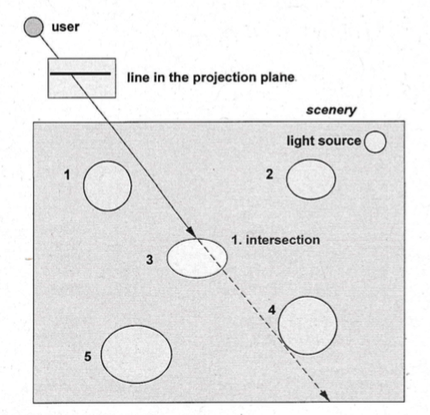
\includegraphics[width=\linewidth]{3_120}
	\end{subfigure}
	\begin{subfigure}[b]{0.3\textwidth}
		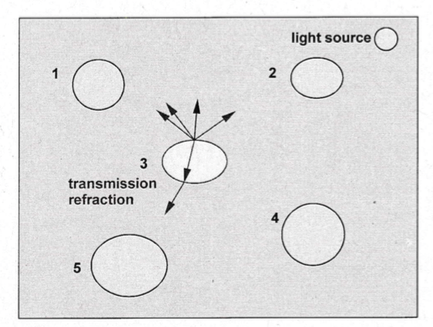
\includegraphics[width=\linewidth]{3_121}
	\end{subfigure}
	\begin{subfigure}[b]{0.3\textwidth}
		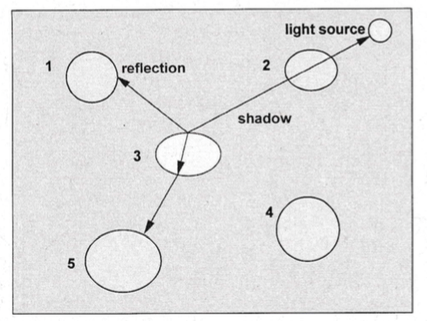
\includegraphics[width=\linewidth]{3_122}
	\end{subfigure}
\end{figure}

\begin{figure}[H]
	\centering
	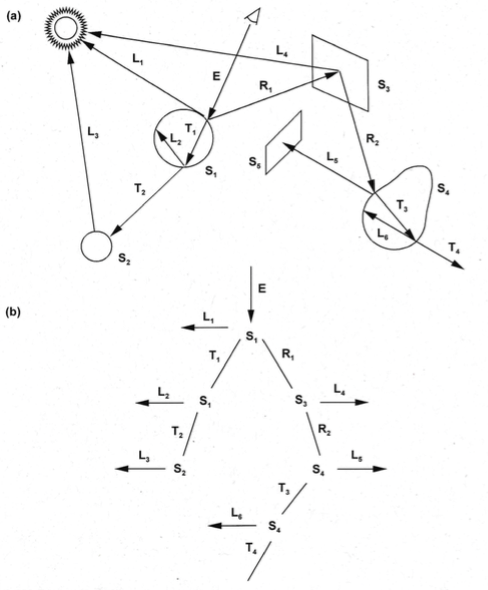
\includegraphics[width=0.7\linewidth]{3_123}
\end{figure}


\setcounter{subsubsection}{4}
\subsubsection{Radiosity}

\begin{itemize}
	\item how light (energy) is distributed in a virtual scenery?
	\item assumption: energy stays constant in a closed room 
		\begin{itemize}
			\item energy radiated from a surface = radiation (or radiosity)
			\item surface is assumed to be an opague, diffuse Lambert. 
		\end{itemize}
	\item radiosity equation: energy leaving is the sum of emiited and reflected light
		\begin{equation}
			B_i = E_i + \rho_i \sum_{i \leq j \leq n} B_j F_{j-i} \frac{A_j}{A_i}
		\end{equation}
		
		where:
		
		\begin{itemize}
			\item $B_i$, $B_j$ are the radiosities of the surface elements i and j, measured as energy per time unit and surface unit (W/m$^2$)
			\item $E_i$ is the emission rate. $> 0$ for light sources, else $0$
			\item $\rho_i$ is the reflection coefficient ($0 \leq \rho_i \leq 1$)
			\item $F_{j-1}$ is a form factor or configuration factor: the amount of energy, which leaves the element j and arrives at the element i. (shape, orientation and hindrance of both elements)
			\item $A_i$, $A_j$ are the areas of i and j
			\item $N$ is the amount of surface elements in a scenery.
		\end{itemize}
	\item approximation of the form factors: semi-cubes or hemispheres are used. (Figure 3.128)
	\item IMPORTANT read the page 3-108 to 3-115 carefully. (interaction steps)
		\begin{enumerate}
			\item iter1: light source emits light $\rightarrow$ go to patches
			\item iter2: patches exposed to the light now emitts light $\rightarrow$ go to another patches
			\item $\dots$
			\item iter16: no more changes after 16 iterations (termination)
		\end{enumerate}
		
		\item form factors
			\begin{itemize}
				\item complex geometry of scene is altered by simplified geometry (mapping)
				\item hemisphere
					\begin{itemize}
						\item fish-eye perspective
						\item center of the hemisphere is the patch 
						\item difficult to deform the image in a fish-eye perspective (computationally expensive)
					\end{itemize} 
				\item semi-cube
					\begin{itemize}
						\item alternative of hemisphere 
						\item drawback: object originally at the same distance from the patch are distorted (objects at the edges) and object at the edges emits more light $\rightarrow$ correction is needed
						\item corrections: geometrical + illumination (with Lambert Law) - mask is used (multiplier)
					\end{itemize}
			\end{itemize}
\end{itemize}

\subsection{Textures}

\begin{itemize}
	\item why texture? 
		\begin{itemize}
			\item creating \textbf{realistic obj}.
			\item creating \textbf{surface properties}
			\item visualize contours
			\item distinguish between different parts of an obj.
		\end{itemize}
	\item two methods for realistic 3D object
		\begin{itemize}
			\item model the unevenness of the object completely. (modeling texture)
				\begin{itemize}
					\item all details are modeled seperately and combined. 
					\item superior realism
					\item huge computing effort (for everytime when the view point changes)
				\end{itemize}
			\item pretend the unevenness with an image (texture mapping)
				\begin{itemize}
					\item reduces calculation
					\item if large angle between the viewing angle and the perpendicular or zoom-in $\rightarrow$ not realistic
				\end{itemize}
			\item should be carefully decided (e.g. if the object is far, texture is more reasonable)
		\end{itemize} 
	\item conclusion: complex object (e.g. golf ball) needs large amount of polygons and if surface properties should be visualized $\rightarrow$ texture is an efficient alternative
	\item classification of textures
		\begin{figure}[H]
			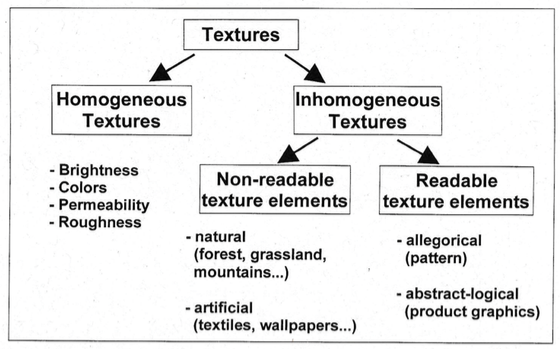
\includegraphics[width=\linewidth]{3_150}
		\end{figure}
	\item issues:
		\begin{itemize}
			\item how to create
				\begin{itemize}
					\item designing texture manually
					\item mathematical methods
				\end{itemize}
			\item how to map
		\end{itemize}
\end{itemize}

\subsubsection{The Different Kinds of Textures}

\begin{itemize}
	\item classification 
		\begin{itemize}
			\item 2D vs 3D
			\item texture defines the changes in color and intensity of the object's surface
		\end{itemize}
\end{itemize}

\subsubsection*{Bump Mapping}

\begin{itemize}
	\item within a bump map, the amount is stored by which the normals are changed towards the perpendiculars of the surfaces. (2D geometry is preserved, but normal vectors are changed) - thus no additional polygons
	\item color, intensities are not changed (thus color change should be saved separately)
	\item \textbf{bump map: array of shift values.} 
	\item \textbf{Bump-Mapping cannot be combined with color interpolation illumination models}: Phong, Raytracing (o) Gouraud (x) (After G., everything is changed into flat)
\end{itemize}

\subsubsection*{3D Texture}

\begin{itemize}
	\item the textures on the surface of the object are a result of the \textbf{several cuts} in the 3D texture space.
\end{itemize}

\begin{figure}
	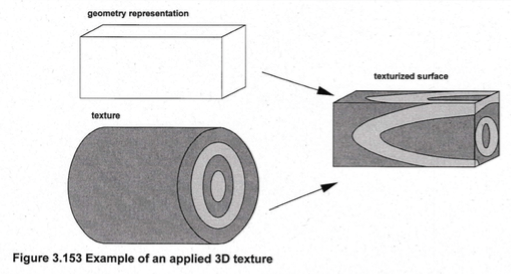
\includegraphics[width=\linewidth]{3_153}
\end{figure}

\subsubsection{The Mapping of Textures}

\begin{itemize}
	\item terms:
		\begin{itemize}
			\item texture plane: 2D plane in which the texture is defined
			\item object space: within 3D object space, the models are created that will be provided later with textures
			\item image field: contains the 2D completely rendered scenery
		\end{itemize}
\end{itemize}

\subsubsection*{Texture Mapping}
       
\begin{itemize}
	\item texture mapping process: from the texture plane (u, v) into 3D object space (r, s, t)$\rightarrow$ from the object space into the 2D image field.
	\item calculating pixel position: positions of a pixel in the image field $\rightarrow$ object space (r, s, t)$\rightarrow$ texture plane (u, v)
		\begin{enumerate}
			\item start from the pixel. 
			\item rectangular (or quadratic) pixel area (4 corner of one pixel) onto the object's surface (if the object surface is not parallel to the monitor surface, mapping defines an amount of points in the object's (r, s, t) coordinate system)
			\item map (r, s, t) to (u, v) (4 points) 
			\item (u, v) points in the pattern defines a quadrangle. 
			\item value for pixel is calculated by adding all texel values in the defined quadrangle. (if (u, v) is outside the texture map, the pattern simply repeated)
		\end{enumerate}
	\item texels: individual elements of the texture image.
		\begin{itemize}
			\item multiple texels could be mapped onto one pixel
		\end{itemize}
	\item time consuming. (not real time)
\end{itemize}

\begin{figure}[H]
	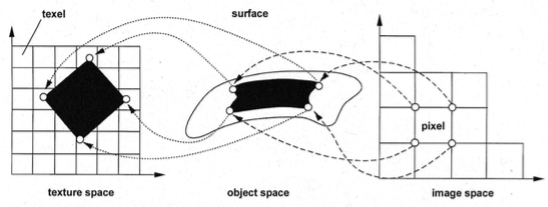
\includegraphics[width=\linewidth]{3_154}
\end{figure} 

\subsubsection*{2-Phase Texture Projection}

\begin{itemize}
	\item if a texture is mapped onto neighboring surface element: junction line between two surfaces is not noticed.
	\item solution:
		\begin{enumerate}
			\item texture firstly mapped onto a simple geometry which surrounds the object (intermediate surface mapping) 
			\item texture is mapped onto the inside of the surrounding geometry
			\item from surrounding to every point of the object.
		\end{enumerate} 
	\item simple geometries for intermediate surfaces: spheres, cones, cylinders, cubes
\end{itemize}       

\begin{figure}[H]
	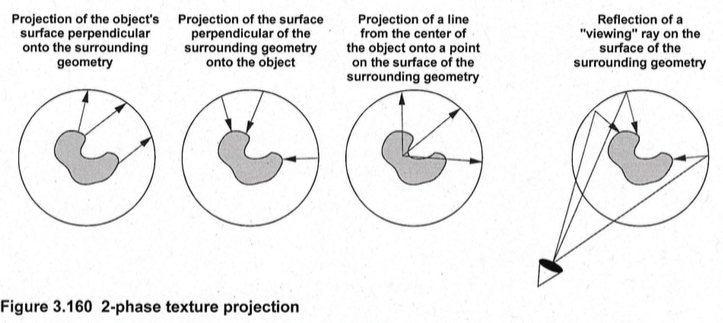
\includegraphics[width=\linewidth]{3_160}
\end{figure} 

\subsubsection*{2-Phase Projection onto a cylinder}

\begin{align}
	x &= r \sin (u \cdot 2 \cdot \theta) \\
	y &= v \\
	z &= r \cos (u \cdot 2 \cdot \theta)
\end{align}

\begin{align}
	u &= \frac{\arcsin \big( \frac{x}{r} \big)}{2 \cdot \theta} \\
	v &= y 
\end{align}

\begin{itemize}
	\item where $r$ is the radius and $\theta$ ($0 \leq \theta \leq 2\pi$) is the angle of the z-axis. u, v is ($0 \leq u, v \leq 1$)
	\item procedure can only be used for dedicated geometries. (if not, large distortion)
\end{itemize}


\subsubsection*{2-Phase Projection onto a sphere}

\begin{align}
	x &= r \sin \theta \cos \phi = r \sin (v \cdot \pi) \cos (u \cdot 2 \cdot \pi) \\
	y &= r \sin \theta \sin \phi = r \sin (v \cdot \pi) \sin (u \cdot 2 \cdot \pi) \\
	z &= r \cos \theta = r \cos (v \cdot \pi)
\end{align}

\begin{align}
	v &= \frac{\arccos \big( \frac{z}{r} \big) }{\pi} \\
	u &= \frac{\arccos \big( \frac{x}{r \cdot \sin (v \cdot \pi) } \big)}{2 \cdot \pi} 
\end{align}

\subsubsection*{Environment Mapping}

\begin{itemize}
	\item approximation using a surrounding geometry differs from the other procedures, because it depends on the location of the user.
	\item object behaves like an ideal mirror. (reflects the environment)
	\item object surface = own texture + texture of environment (environment is not static but changes) 
	\item Types:
		\begin{itemize}
			\item spherical 
			\item dual paraboloid
			\item cubic
		\end{itemize}
\end{itemize}

\begin{figure}[H]
	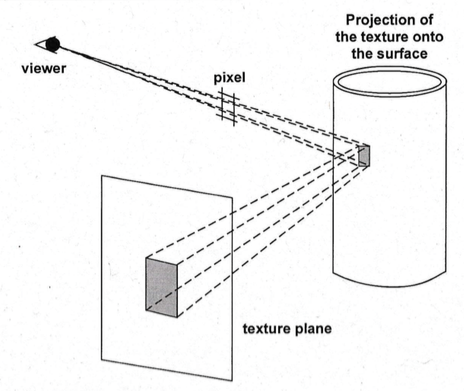
\includegraphics[width=\linewidth]{3_164}
\end{figure} 

\subsubsection*{Spherical environment mapping}

\begin{itemize}
	\item whole env. is projected into the inside of a sphere.
	\item only works if the object that has to be mapped by the texture does not change its position. (if not, complete surrounding texture should be recalculated)
	\item can be supported by graphics card 
	\item read the page 3-127 to 3-128
\end{itemize}

\subsubsection*{Dual Paraboloid}

\begin{itemize}
	\item mapping uses two textures: back texture + front texture (rectangular but parabolically distorted)
	\item independent of the user's viewpoint (than spherical env mapping)
	\item but textures are difficult to generate.
\end{itemize}

\subsubsection*{Cubic Environment Mapping}

\begin{itemize}
	\item instead of applying only one texture, map six different sides, which are placed around the object like a large cube
	\item in principal, is not restricted to one viewpoint. (realistic but computationally expensive)
	\item more correct reflection of the environment, but is not completely correct since some distortion could apprear at the edges and corners due to an imprecise calculation. 
\end{itemize}
      
\end{document}